\section*{Pavages par des triominos}

On revient ici sur les pavages par des triominos (cf. 5. de l'exercice 1) de grilles (ici, complètes) $a \times b$ rectangulaires, puis carrées, sur lesquels on se pose des questions complémentaires.

Il est recommandé de dessiner sur sa copie les grilles au stylo, mais les triominos au crayon de papier. On pourra s'aider, comme brouillon, des grilles déjà tracées figurant dans l'énoncé.


\medskip

\begin{center}
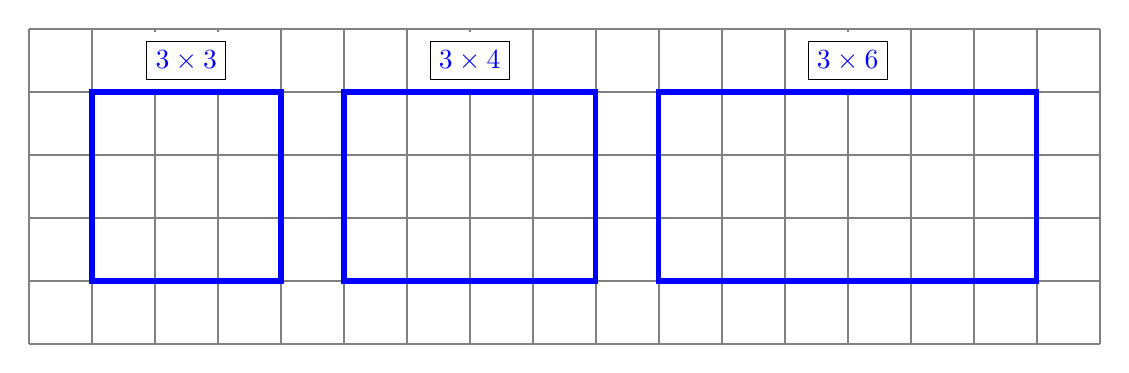
\begin{tikzpicture}[scale=0.8]
    % Dimensions : 10 colonnes (x) et 17 lignes (y)
\def\rows{5}
\def\cols{17}
\def\cell{1} % taille d'une case en cm

% Dessiner la grille grise
\draw[gray, step=\cell, thick] (0,0) grid (\cols*\cell, \rows*\cell);
\draw[line width=2pt, blue] (1,1)--(4,1) -- (4,4) -- (1,4) -- cycle;
\node[fill=white] at (2.5,4.5) {\fbox{\textcolor{blue}{$3\times 3$}}}; 
\draw[line width=2pt, blue] (5,1)--(9,1) -- (9,4) -- (5,4) -- cycle;
\node[fill=white] at (7,4.5) {\fbox{\textcolor{blue}{$3\times 4$}}}; 
\draw[line width=2pt, blue] (10,1)--(16,1) -- (16,4) -- (10,4) -- cycle;
\node[fill=white] at (13,4.5) {\fbox{\textcolor{blue}{$3\times 6$}}}; 
\end{tikzpicture}
\end{center}


\begin{enumerate}
\item Représenter un pavage d'une grille dans le cas où $a = 3$ et $b = 4$.



\item \begin{enumerate}
\item On suppose que l'on peut paver une grille de taille $a \times b$ (on la dit alors « pavable »). Montrer que l'entier $ab$ est divisible par 3.



\item Trouver la plus petite grille carrée pavable de taille $a \times a$.



\item La condition « $ab$ est divisible par 3 » est-elle suffisante pour garantir qu'une grille de taille $a \times b$ soit pavable ?


\end{enumerate}

\item On suppose que $a = 2$. À quelle condition nécessaire et suffisante sur $b$ une grille de taille $2 \times b$ est-elle pavable ?



\item Travaux manuels.

Sur l'un des bandeaux $2 \times 16$ ci-dessous, on a symétrisé le triomino encré en noir par rapport à l'axe $\Delta_1$, cela a donné le triomino teinté en clair à l'autre bout. On symétrise ce nouveau triomino par rapport à l'axe $\Delta_2$, puis le nouveau-nouveau triomino par rapport à $\Delta_3$.


\begin{center}
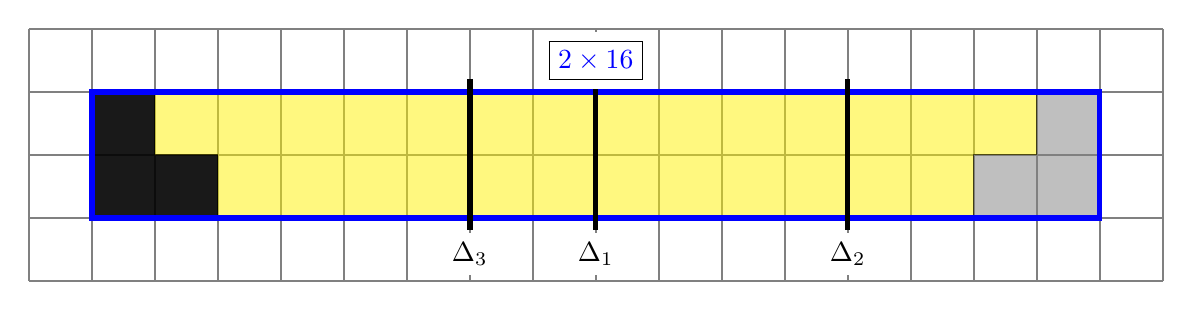
\begin{tikzpicture}[scale=0.8]
    % Dimensions : 10 colonnes (x) et 17 lignes (y)
    \def\rows{4}
    \def\cols{18}
    \def\cell{1} % taille d'une case en cm
    
    % Dessiner la grille grise
    \draw[gray, step=\cell, thick] (0,0) grid (\cols*\cell, \rows*\cell);
    
    % Optionnel : entourer la grille d'un trait plus épais
   % \draw[thick] (0,0) rectangle (\cols*\cell, \rows*\cell);
 \begin{scope}[shift={(3,1)}]
 \draw[rotate=90,fill=black, opacity=0.9] (0,0) -- (1,0) -- (1,1) -- (2,1) -- (2,2) -- (0,2) -- cycle;
 \end{scope}
 
 % L n°3 : rotation 180°
 \begin{scope}[shift={(17,3)}]
 \draw[rotate=180,fill=gray, opacity=0.5] (0,0) -- (1,0) -- (1,1) -- (2,1) -- (2,2) -- (0,2) -- cycle;
 \end{scope}
 
 \begin{scope}[shift={(2,1)}]
  \draw[fill=yellow, opacity=0.5] (0,2) -- (14,2) -- (14,1) -- (13,1) -- (13,0) -- (1,0) -- (1,1) -- (0,1) -- cycle;
  \end{scope}
  
  \draw[line width=2pt, blue] (1,1)--(17,1) -- (17,3) -- (1,3) -- cycle;
  
 \draw[line width=2pt, ] (7,3.2)--(7,0.8) node[fill=white,below] {$\Delta_3$};
 
\draw[line width=2pt, ] (9,3.2)--(9,0.8) node[fill=white,below] {$\Delta_1$};

\draw[line width=2pt, ] (13,3.2)--(13,0.8) node[fill=white,below] {$\Delta_2$};

\node[fill=white] at (9,3.5) {\fbox{\textcolor{blue}{$2\times 16$}}};
\end{tikzpicture}
\end{center}


\begin{enumerate}
\item Dessiner sur votre copie à l'échelle $1/2$ le bandeau et les 4 triominos (dont celui d'origine) en présence.



\item Découper un bandeau (à l'échelle 1) de l'énoncé, remplacer chaque symétrie par un pliage en faisant en sorte que le triomino noir soit toujours visible. Enfin découper selon ses traits. On obtient une farandole de 8 triominos identiques. Pourquoi ? \textit{Le deuxième bandeau en fournit aussi 8}.

\begin{center}
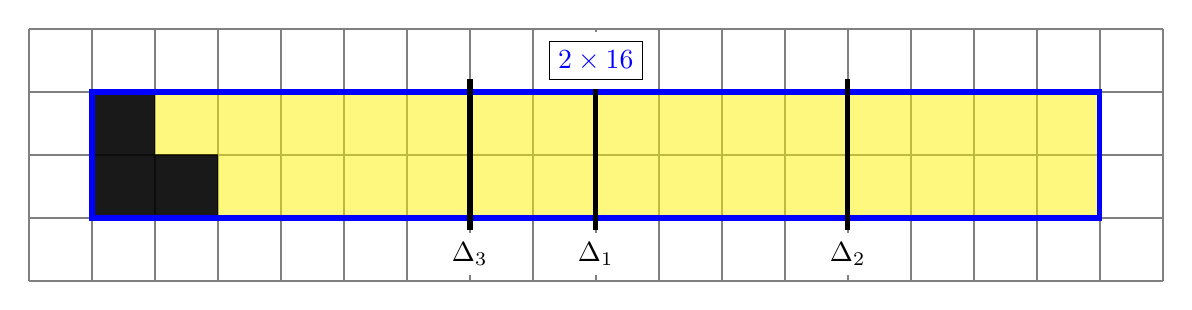
\begin{tikzpicture}[scale=0.8]
    % Dimensions : 10 colonnes (x) et 17 lignes (y)
    \def\rows{4}
    \def\cols{18}
    \def\cell{1} % taille d'une case en cm
    
    % Dessiner la grille grise
    \draw[gray, step=\cell, thick] (0,0) grid (\cols*\cell, \rows*\cell);
    
    % Optionnel : entourer la grille d'un trait plus épais
   % \draw[thick] (0,0) rectangle (\cols*\cell, \rows*\cell);
 \begin{scope}[shift={(3,1)}]
 \draw[rotate=90,fill=black, opacity=0.9] (0,0) -- (1,0) -- (1,1) -- (2,1) -- (2,2) -- (0,2) -- cycle;
 \end{scope}

 
 \begin{scope}[shift={(2,1)}]
  \draw[fill=yellow, opacity=0.5] (0,2) -- (15,2) -- (15,0) -- (1,0) -- (1,1) -- (0,1) -- cycle;
  \end{scope}
  
  \draw[line width=2pt, blue] (1,1)--(17,1) -- (17,3) -- (1,3) -- cycle;
  
 \draw[line width=2pt, ] (7,3.2)--(7,0.8) node[fill=white,below] {$\Delta_3$};
 
\draw[line width=2pt, ] (9,3.2)--(9,0.8) node[fill=white,below] {$\Delta_1$};

\draw[line width=2pt, ] (13,3.2)--(13,0.8) node[fill=white,below] {$\Delta_2$};

\node[fill=white] at (9,3.5) {\fbox{\textcolor{blue}{$2\times 16$}}};
\end{tikzpicture}
\end{center}

\end{enumerate}
\newpage
\item On suppose dans cette question que $a = 5$. On s'aidera au besoin des 16 petits triominos qu'on disposera sur les grilles ad-hoc pour ses tests au brouillon.

\begin{enumerate}
\item Représenter un pavage convenable d'une grille quand $b = 6$.



\item Représenter un pavage convenable d'une grille quand $b = 9$.

\begin{center}
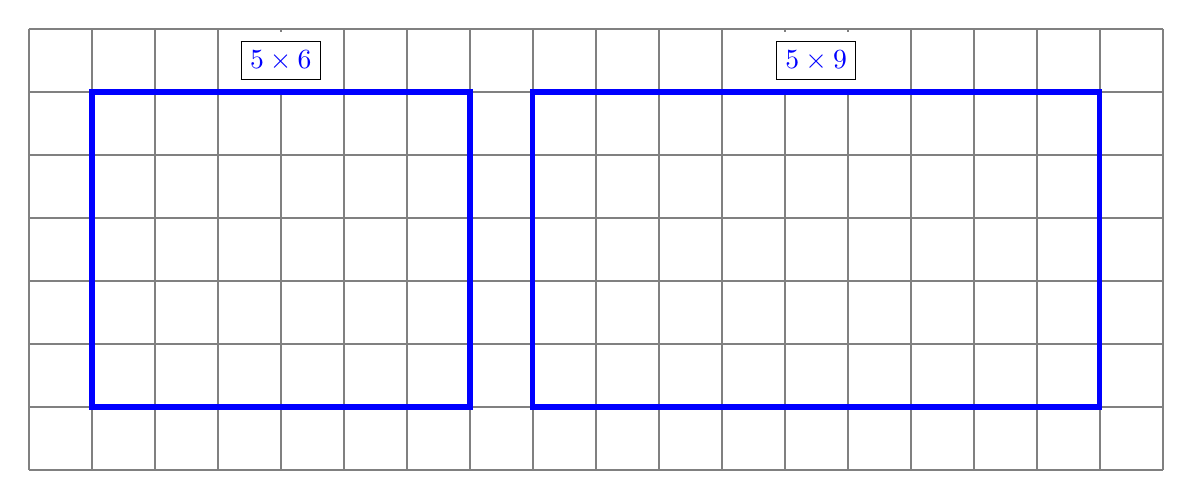
\begin{tikzpicture}[scale=0.8]
    % Dimensions : 10 colonnes (x) et 17 lignes (y)
\def\rows{7}
\def\cols{18}
\def\cell{1} % taille d'une case en cm

% Dessiner la grille grise
\draw[gray, step=\cell, thick] (0,0) grid (\cols*\cell, \rows*\cell);
\draw[line width=2pt, blue] (1,1)--(7,1) -- (7,6) -- (1,6) -- cycle;
\node[fill=white] at (4,6.5) {\fbox{\textcolor{blue}{$5\times 6$}}}; 
\draw[line width=2pt, blue] (8,1)--(17,1) -- (17,6) -- (8,6) -- cycle;
\node[fill=white] at (12.5,6.5) {\fbox{\textcolor{blue}{$5\times 9$}}}; 

\end{tikzpicture}
\end{center}

\item On suppose $b$ divisible par 3, $b \geq 6$. Montrer que l'on peut paver une grille de taille $5 \times b$.


\end{enumerate}

\item On suppose que $b$ est divisible par 3 et que l'on peut paver une grille de taille $a \times b$. Montrer que l'on peut alors paver une grille de taille $(a + 2) \times b$.



\item On suppose que $a \geq 4$, et $b \geq 4$. Montrer que l'on peut paver une grille de taille $a \times b$ si, et seulement si, $ab$ est divisible par 3. En déduire les grilles carrées que l'on peut paver.


\end{enumerate}
